\chapter{Anhang}

\section{Architekturen}

\begin{figure}
	\centering
	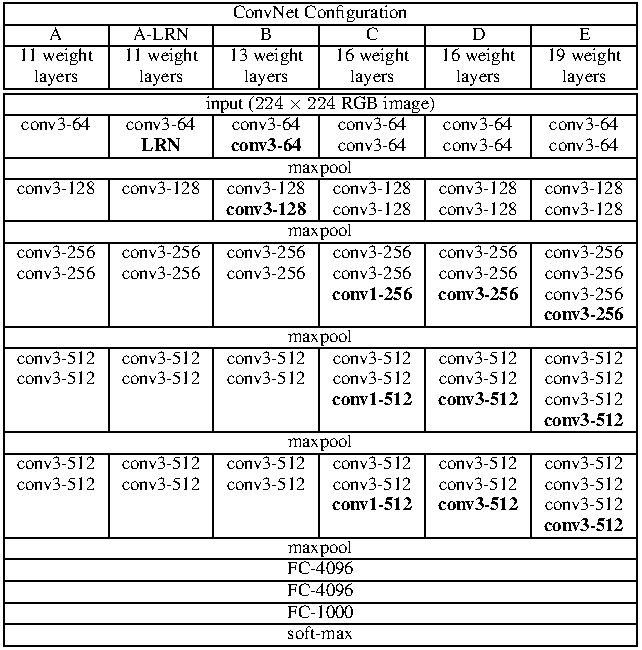
\includegraphics[width=0.8\textwidth]{Bilder/vgg16-architecture.pdf} 
	\caption{Die ursprünglichen VGG-Architekturen. Spalte D zeigt VGG16 wie in \autoref{sec:pretrained-backbones:vgg16} beschrieben. Abb. aus \cite{Simonyan.04092014}.}
	\label{fig:vgg16-architecture}
\end{figure} 

\begin{figure}
	\centering
	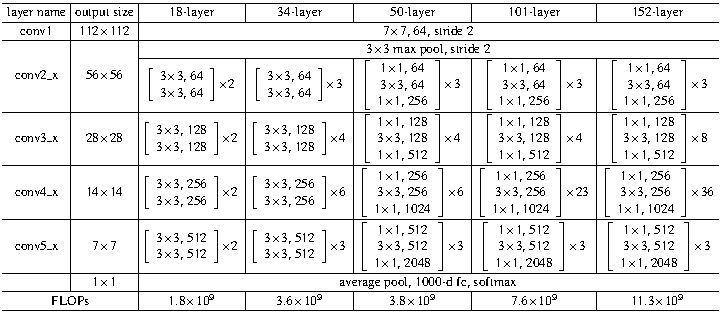
\includegraphics[width=0.8\textwidth]{Bilder/resnet34-architecture.pdf} 
	\caption{Die ursprünglichen ResNet-Architekturen. Zwischen jeweils zwei Convolutional-Layer befindet sich eine Skip-Connection \cite{He.10122015}.}
	\label{fig:resnet34-architecture}
\end{figure} 

\begin{figure}
	\centering
	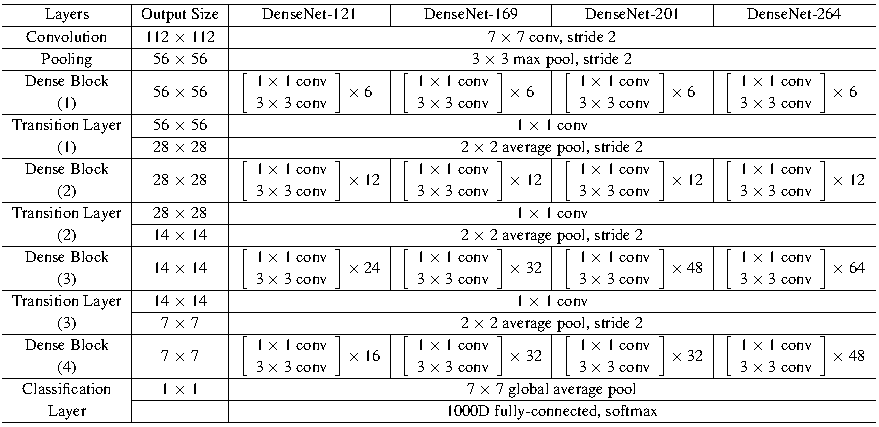
\includegraphics[width=0.8\textwidth]{Bilder/densenet121-architecture.pdf} 
	\caption{Die ursprünglichen DenseNet-Architekturen \cite{Huang.25082016}.}
	\label{fig:densenet121-architecture}
\end{figure} 

\begin{figure}
	\centering
	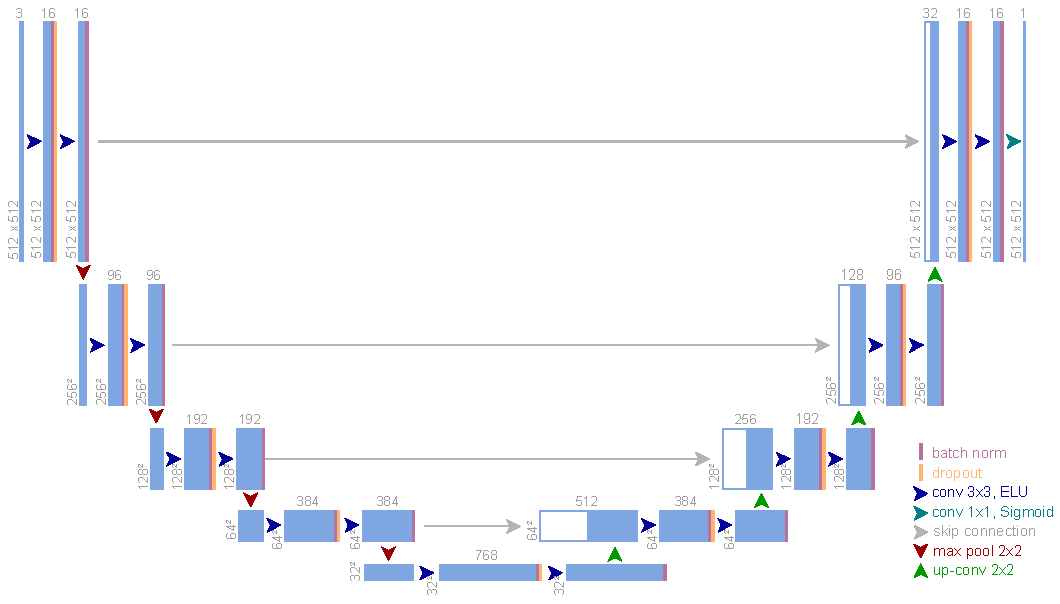
\includegraphics[width=1.\textwidth]{Bilder/own-unet-15mil.pdf} 
	\caption{Bike-U-Net-15 mit 15,165 Mio. Parametern.}
	\label{fig:bike-unet-15}
\end{figure} 

\section{Quelltext-Implementation}

\lstinputlisting[
	label=code:quality,    % Label; genutzt für Referenzen auf dieses Code-Beispiel
	caption=Implementation des Quality-Maßes in Python zur Verwendung im Training und Testen von Keras-Modellen.,
	captionpos=b,               % Position, an der die Caption angezeigt wird t(op) oder b(ottom)
	style=EigenerPythonStyle,   % Eigener Style der vor dem Dokument festgelegt wurde
	firstline=1,                % Zeilennummer im Dokument welche als erste angezeigt wird
	lastline=50                 % Letzte Zeile welche ins LaTeX Dokument übernommen wird
]{Quellcode/quality.py}